\chapter{Comparison and further discussion}

\vspace{-25pt}
This Section reviews and discusses the touch points of the two articles just described, along with a final glance at current policy actions on the topic.
\vspace{-15pt}

\section{Links and notes}
\vspace{-8pt}
We live in a world that is the result of many decades of intensified globalization and internationalization, both economically and culturally. The establishment of international organizations such as the World Trade Organization in 1995 promoted international cooperation and economic integration. Supporting this, the left side of Figure \ref{img:trade} illustrates trade intensity, measured as the sum of exports and imports of goods and services in \% GDP terms, between 1970 and 2021 for three entities. All three, over the years, have opened their economies, moving from being closed~countries~to~open~countries.

\begin{figure}[!h]
    \centering
    \captionsetup{font=footnotesize,justification=centering}\caption{left: time series for trade/GDP, own work on World Bank data\\right: time series for the inverse Quinn index for capital controls intensity, \textcite{klein}}
    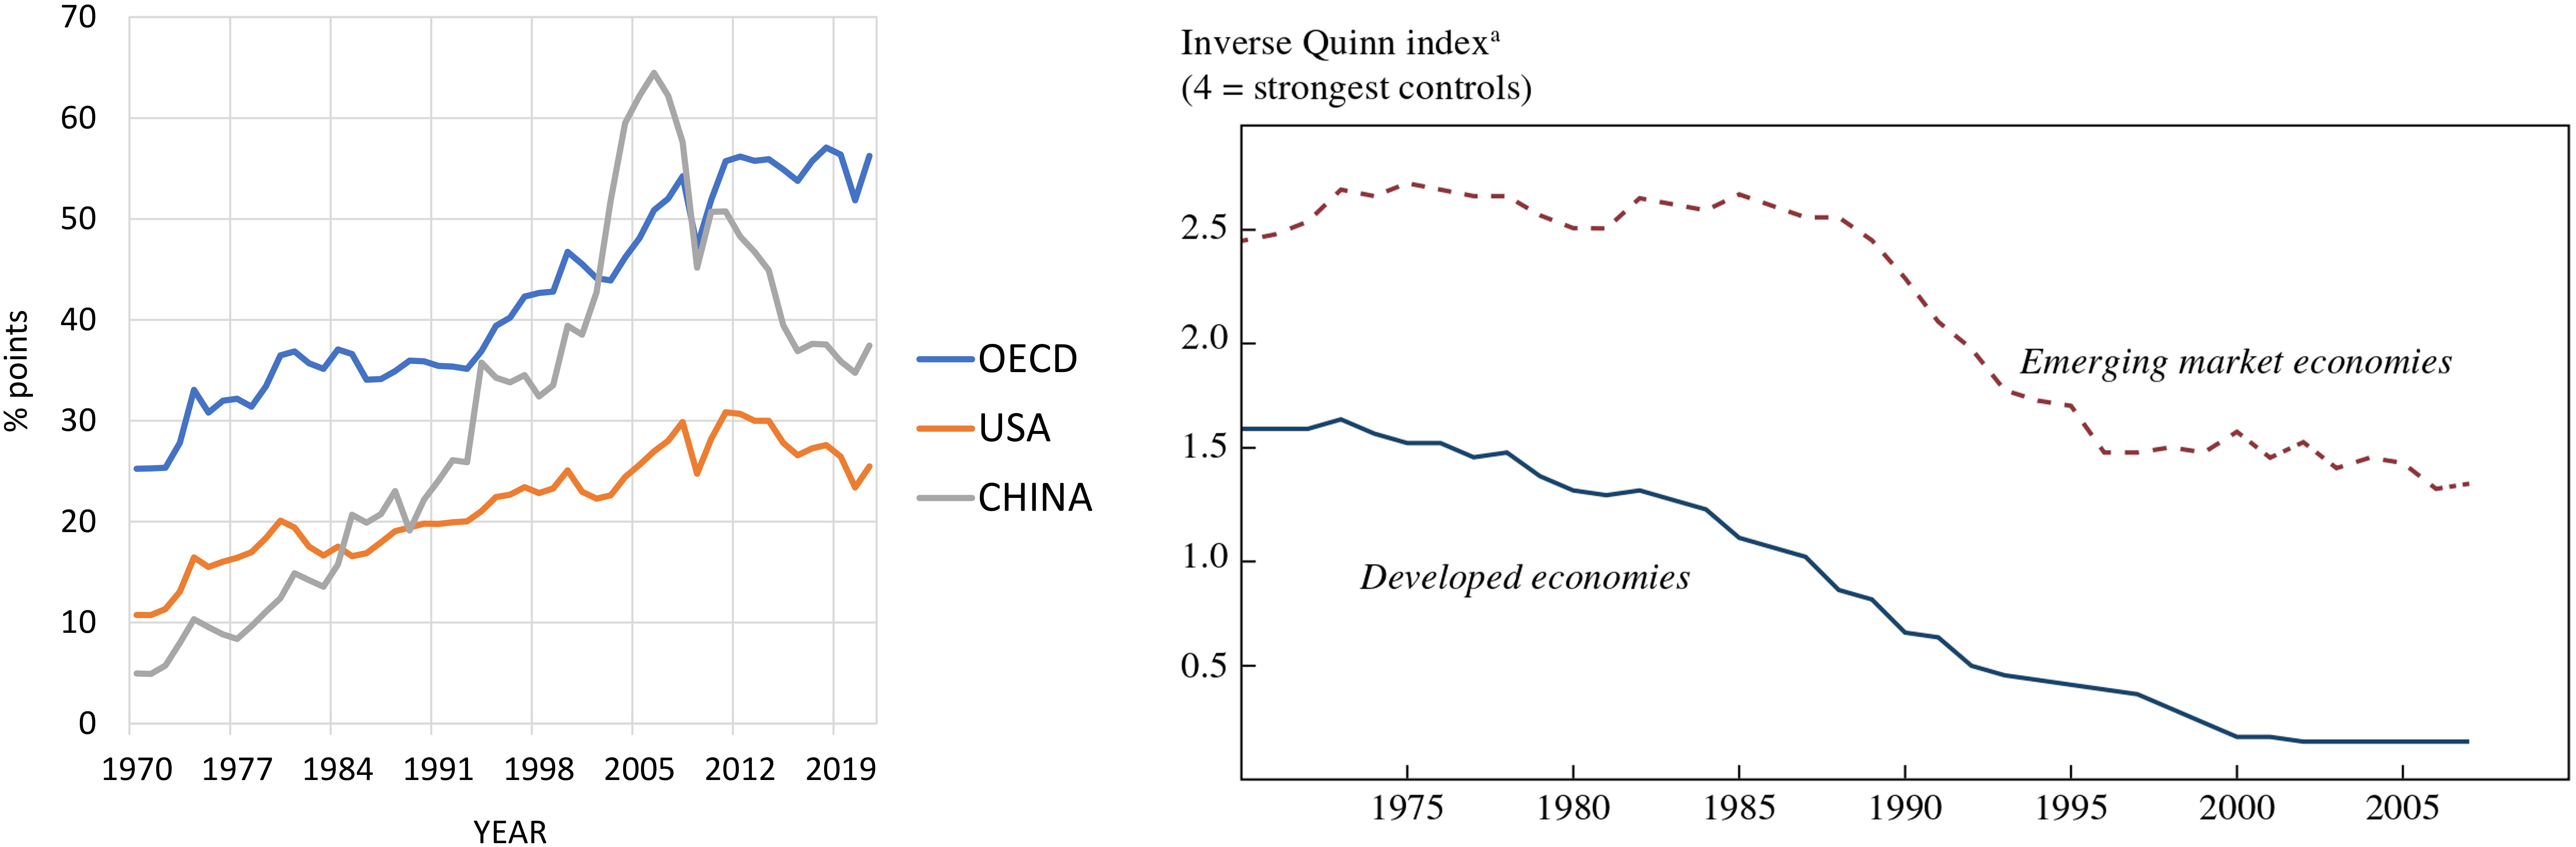
\includegraphics[width=0.65\textwidth]{img/trade-and-controls.jpg}
    \label{img:trade}
    \vspace{-5pt}
\end{figure}

As part of this internationalization process, to encourage capital inflows and facilitate international trade and investments, countries have loosened their capital restrictions. Formalizing and capturing a general measure for capital controls is quite challenging, and most of the literature, including \textcite{dev-loc-red-08}, relies on Quinn's 1997 measure for the intensity of capital controls. On the right side of Figure \ref{img:trade}, it is shown an updated 2011 version of the index, and unquestionably, over time, capital controls have actually been lowered. However, their relaxation also poses risks, such as a higher vulnerability to external shocks, that, in the context of strategic tax interaction, as argued by \textcite{dev-loc-red-08}, leads to a lower corporate income statutory tax rate. While this result is considered a given also in \textcite{clausing}, other authors come to different conclusions. For instance, \textcite{swank-98} rejects the general view that increased capital mobility has directly forced governments to lower their tax burdens and, instead, suggests that tax cuts actually result from a shift in tax policy paradigms.

\begin{figure}[!ht]
    \centering
    \captionsetup{font=footnotesize,justification=centering}\caption{left: time series for avg statutory tax rate 2000-2022, own work on OECD data\\right: time series for corporate income and total tax revenues, own work on OECD data}
    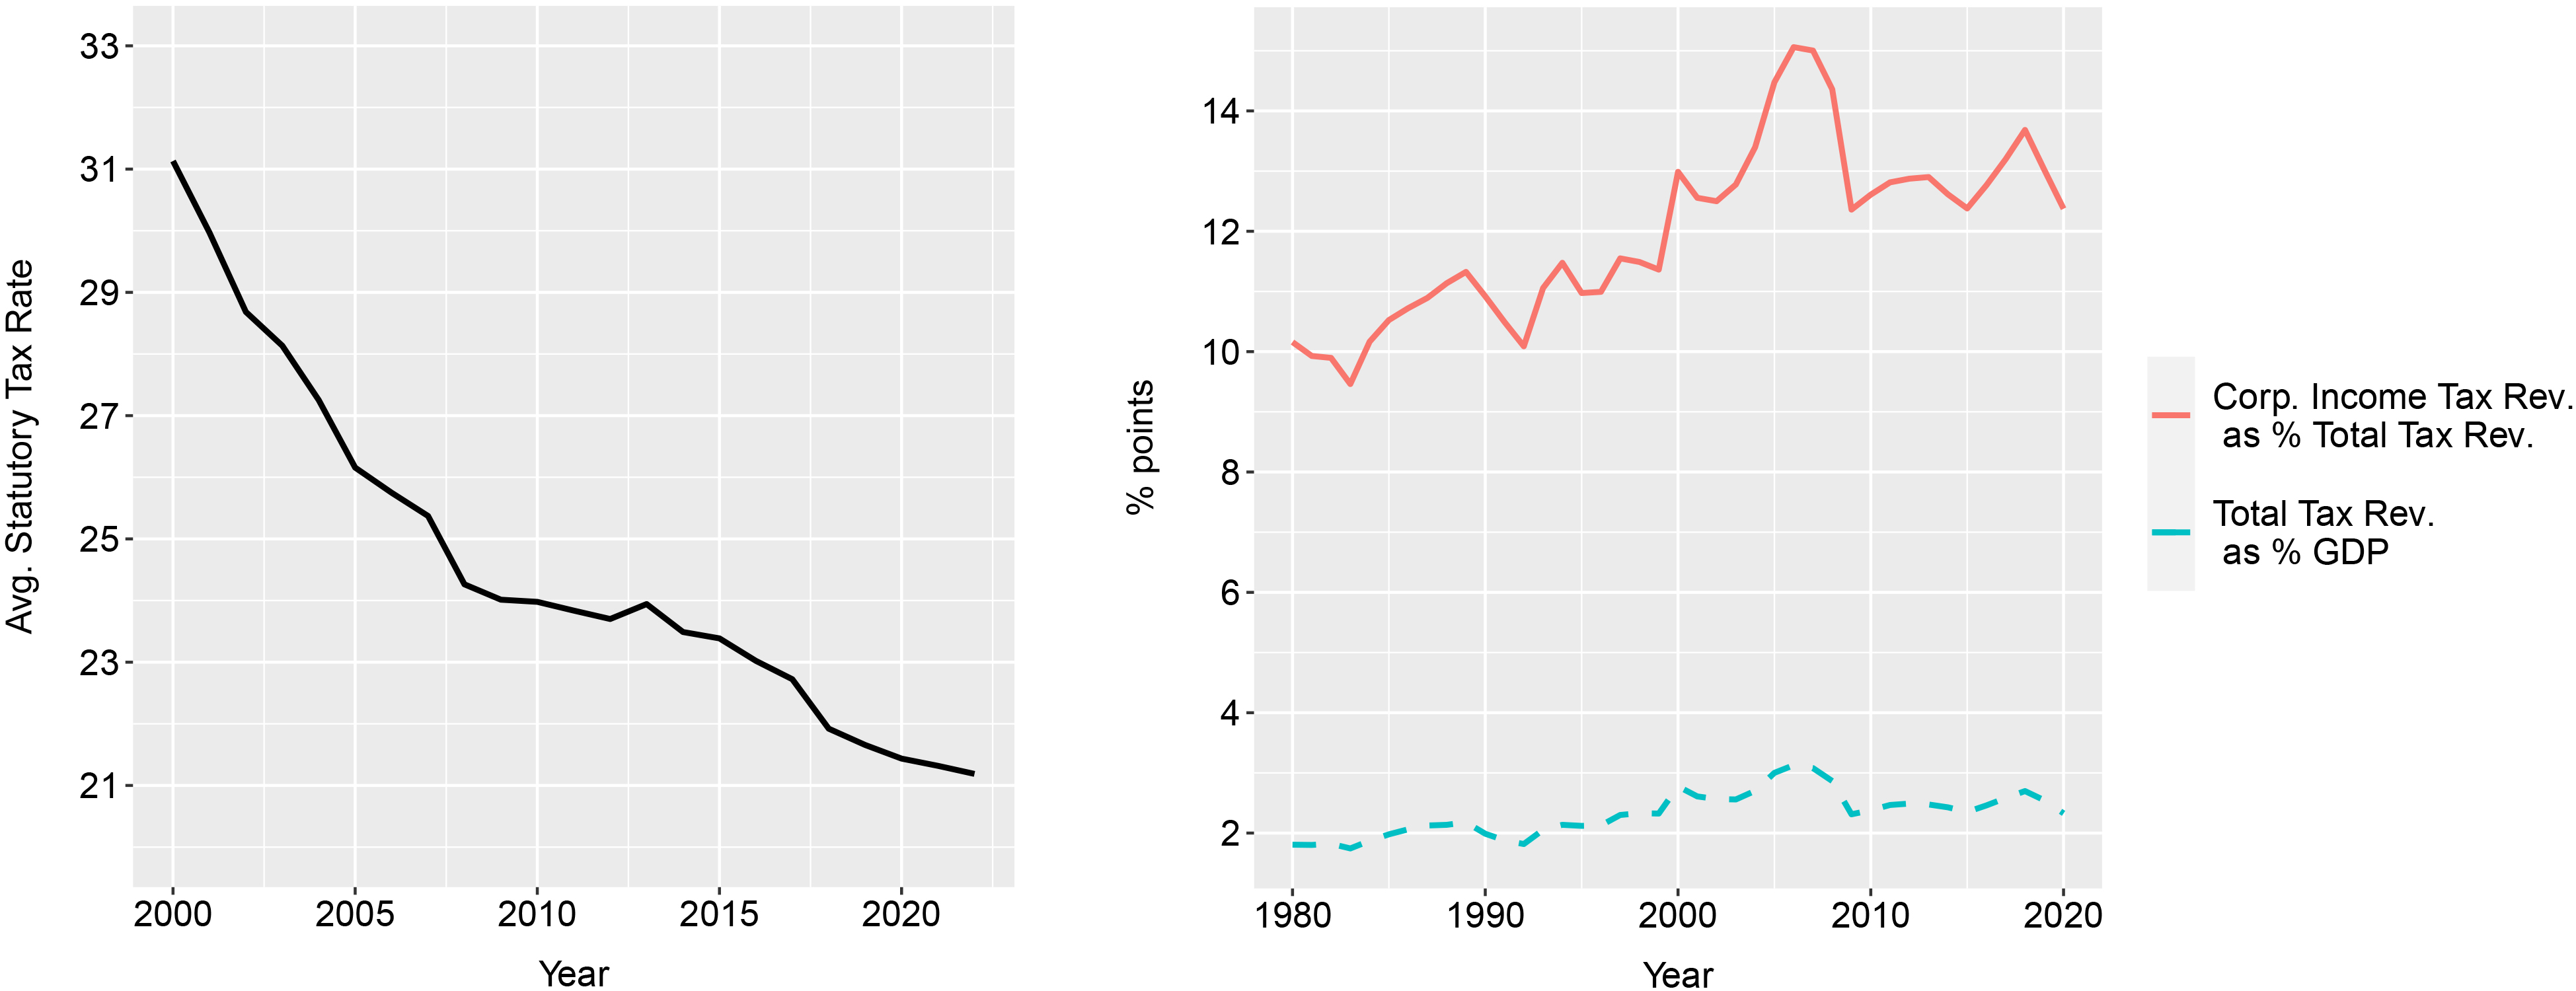
\includegraphics[width=0.65\textwidth]{img/stat-corp.jpg}
    \label{img:stat-revenues}
    \vspace{-5pt}
\end{figure}
Since the analysis of \textcite{dev-loc-red-08} is based on data from only 21 OECD countries between 1982 and 1999, on the left of Figure \ref{img:stat-revenues}, I present an extension of the time series. Using OECD data, I plotted the average corporate income statutory tax rate for 29 OECD states between 2000 and 2022. The fall in tax levels has continued in the last two decades, falling from $31.13\%$ to $21.19\%$. Between 2008 and 2013, the reduction slowed down, and this may be due to stress on governments' fiscal budgets, which were eroded by stimulus measures following the global financial crisis of 2008-2009, ultimately to prevent short-term revenue losses. A particularly weak point of the first paper is that the authors, in order to measure the change in the marginal tax following a change in the capital stock (EMTR), decided to use a simpler measure, the tax wedge. The reason they adopted this alternative variable is that they observed large standard errors using an EMTR index directly. In my opinion, in order to still use the main measure, ultimately obtaining more reliable results, some possible solutions could be as follows. First, increase the sample size by collecting data over a longer period from reliable data sources. Secondly, add lagged variables which can control for autocorrelation and capture the effect of past observations on the current value.

In her paper, \textcite{clausing} estimates a revenue-maximizing corporate income tax rate of around 33\%. Although this result may have been reasonable in the period she analyzed, 1979-2002, current rates are considerably distant from that threshold. In this regard, it would be interesting to investigate what is the current profit-maximizing corporate income tax rate for OECD countries. Despite that, with such low tax rates, how can governments continue to provide public goods? Firstly, both \textcite{dev-loc-red-08} and \textcite{clausing} agree that, over time, policymakers have broadened tax bases by eliminating tax exemptions and reducing deductions or credits. Secondly, as modelled by \textcite{clausing}, a tax cut inevitably reduces fiscal revenues as a direct effect but also triggers firms' reaction, in terms of their strategic decisions, profitability and size. Lastly, the right side of Figure \ref{img:stat-revenues} illustrates the size and trend for corporate income tax revenues in GDP terms and as a ratio over total tax revenues. The data regards 29 OECD countries between 1980 and 2020 and shows how, in the end, the tax base widening has fully offset the direct loss of tax cuts. Furthermore, tax revenues generated from corporate income represent only a small portion~of~the~whole,~only around 12\%, while more significant is the contribution coming from personal income taxes.

\vspace{-10pt}
\section{Policy intervention}
\vspace{-10pt}

To conclude, here is a glimpse into the future of international taxation. So far, to explain the fall in corporate income tax rate, we modelled tax competition as a strategic "game". However, in the real world, this interaction on tax rates between countries may be hostile, clashing with political and economic interests. A well-known example is the existence of tax havens, even within OECD and EU jurisdictions (such as Ireland and Hungary, with a CIT of 12.5\% and 9\%, respectively), to which firms shift their profits to benefit from the more favourable taxation. Nevertheless, on a large scale, this phenomenon brings fairness problems to the system since, for instance, the law generally requires profits to be taxed in the country where they are generated. With this in mind, since 2013, OECD has intensified its tax coordination efforts with the ambitious Base Erosion Profit Shifting (BEPS) two-pillar project. Among the others, Pillar Two of this directive introduces a global minimum tax of 15\% on profits of organizations, and their subsidiaries, that have a consolidated group revenue over €750 mln. Having said that,  and recalling the assumptions and results of \textcite{dev-loc-red-08}, it would be interesting to investigate the consequences of the global minimum tax over the statutory tax levels. To my mind, the introduction of such a low tax rate, indeed lower than the current average in the OECD area, will likely increase the tax burden in jurisdictions where the rate is below 15\%. Clearly, for states joining the pact, having a tax rate below the 15\% threshold would no longer be worthwhile, as the revenues generated by the difference between the two tax rates would be redistributed to other countries. On the other hand, countries with a higher tax burden than 15\% may act ambiguously or more likely not react. In this way, they would still apply higher tax rates to companies not concerned by the BEPS and hopefully gain new revenues from the new directive.